\documentclass{article}
\usepackage[utf8]{inputenc}
\usepackage{graphics}
\title{%
  Trackzheimers \\
  \large  Alzheimer’s Disease progression tracking app}

\author{Alva Annett\\Erik Bürger \\ Abhishekapriya Ganesan\\Raphaela Pensch\\Aina Vaivade}
\date{30 January 2020}

\usepackage{natbib}
\usepackage{graphicx}

\begin{document}

\maketitle

\section{Introduction}
\subsection{What is Trackzheimers}
The aim of the web application that we are developing is to help both Alzheimer's Disease patients,and their doctors to track the progress of Alzheimer's symptoms in the patient. This is done by allowing the patients to take continuous memory tests through the web application in between visits at their physician. Hence the doctors will be able to monitor the patients mental state and progress continuously through the web application. In this way the doctors will have a better picture of his/hers patients mental state and progress.\newline
\newline If there is time, we will also add the option to add an account for the patients caregivers or relatives, through which they can help the patient to remember to take the tests continuously. Through their account they will be able to get an alert if the patient has forgotten to take the memory test.\newline
\newline In this web application there will also be the possibility to create an account as a researcher. The researchers will only have access to anonymized patient data, which they can use in their own research. % I would like to add something more to this but I got stuck. %

\subsection{What is Alzheimer's Disease}
% Short description of Alzheimer's%

\subsection{Are there similar web applications already?}
% Maybe we could add a section about similar products, just to clarify how this web application duffers from other products% 

\section{System architecture}
%Maybe we could describe how we think that we will build the system and what we have done so far. We could also include problems and issues that we might have or have had%

\begin{figure}
    \centering
    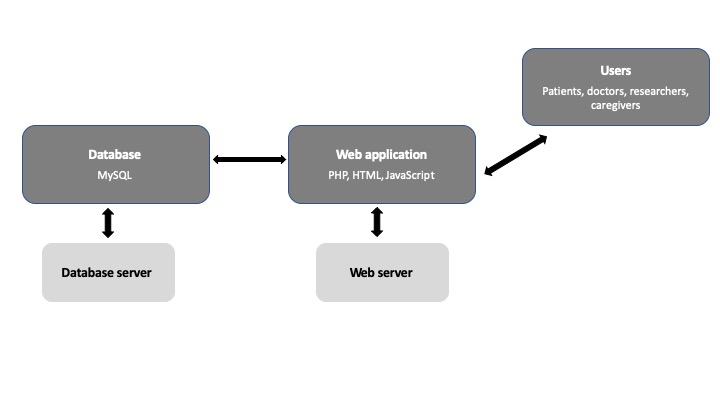
\includegraphics[scale=0.5]{report/System_arch.jpg}
    \caption{System architecture of the web application Trackzheimers. Included are some of the programming languages we are using in the different parts. }
    \label{fig:system_arch}
\end{figure}

The basic system architecture for this web application is illustrated in figure \ref{fig:system_arch}. The database is located in the database server and is where we store all the data, for example user information and memory tests. Data travels back and forth continuously from the database to the web application. The web application is where the user interface is, meaning everything that interacts with the different users. Depending on what kind of user you are you have different rights to add or read different things from the database. For example caregivers do not have access to patient information, only to know if the patient that he or she is connected to has taken the memory test or not. When programming the web application we use PHP, HTML and JavaScript. PHP is used for the back end development of the web application, while JavaScript is for the front end. 

\subsection{What we have done so far}
When starting to build this web application we decided to start with making an ER diagram, which we than use to build the database. The ER diagram you can see in Appendix A, and it contains more than what the database contains at this moment. Since we wanted to build a basic web application that works as fast as possible, which we than can continue with and building on, we decided to start with two user groups; doctors and patients. The idea is to the other user groups (researchers and caregivers) as we go when we have a working basic web application. \newline
\newline We have also started with the HTML files for the web application in general, as well as for both user groups (doctors and patients). These HTML files have the basic functions that the web application will need, and also here we will continue to develop and add functions to it as we go. The basic general HTML files that we have created are the starting page, which also is the log in page, a page for registration, an information page and a contact page. General for all pages is that they have a navigation bar at the top, so that the users easily can go from one page to the other. Since our main target group is Alzheimer's Disease patients we have chosen to make the page design as easy as possible, and it is also the reason why we decided to have the login page as the home page. The HTML files special for the patient user-group are the tests and their statistics, as well as their profile page. Note that the HTML files for the test are not completed yet. For the doctors we have created a specific starting page, a profile page and a page where they can search for their patients.\newline
\newline Some of the HTML files that we have created needs further work until they will have all the basic functionalities. This work is for example to connect them to the database so that they either can add data to it or fetch data from the database. For example the registration page needs to be connected to the database so that patient accounts or doctor accounts can be created. The search page that the doctors have needs to be connected to the database so that the search function can be enabled, and more.

\subsection{Further work}
The next step is to connect every HTML file to each other as well as to the database when necessary. We also need to finish creating the memory test. After this we sill have a basic working web application that we can continue working on and add on other functionalities.\newline
\newline If we have the time we will also add two more user groups; the researchers and the caregivers or relatives. Furthermore we will also add memory games to the patients page so that they can play different memory games as well and not only take the memory game through this web application. 

\bibliographystyle{plain}
\bibliography{references}

\newpage
\appendix
\section{ER diagram}
\begin{figure}[h!]
    \centering
    \rotatebox{90}{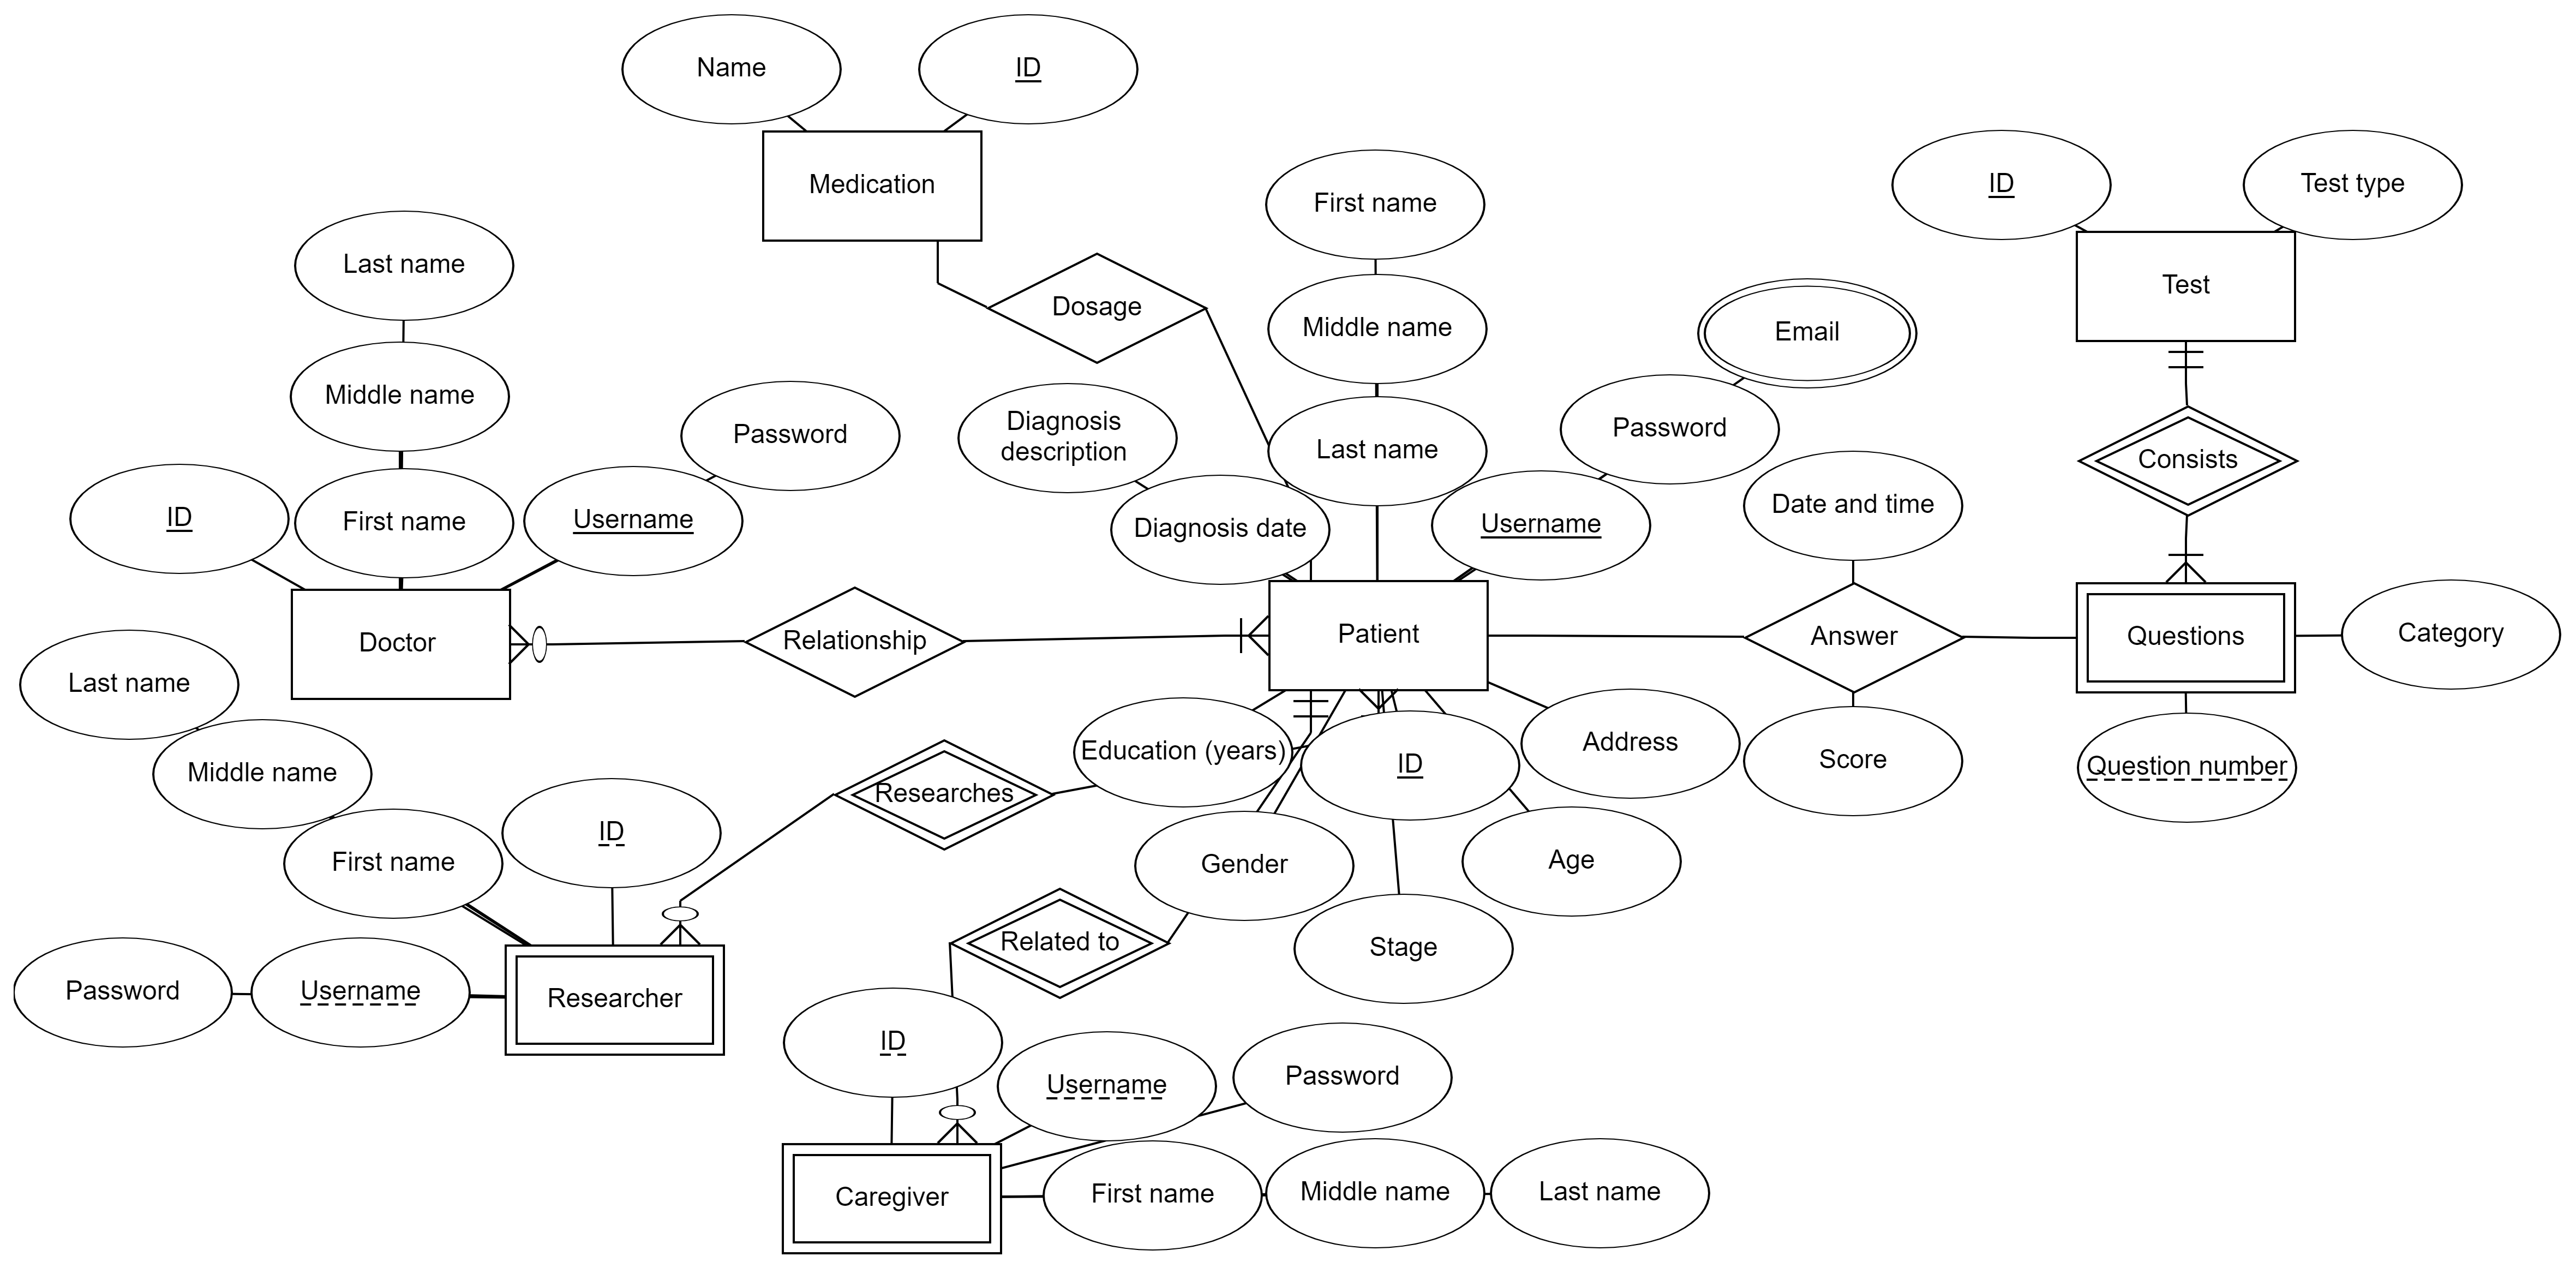
\includegraphics[width=1.4\textwidth]{report/IMS_AlzheimersERD.png}}
    \caption{ER diagram for our database.}
    \label{fig:ER-diagram}
\end{figure}

\end{document}
